\documentclass{beamer}

\usepackage{array}
\newcolumntype{M}[1]{>{\centering\arraybackslash}m{#1}}
\newcolumntype{N}{@{}m{0pt}@{}}

\usetheme{default}
\usecolortheme{rose}
\usepackage{hyperref}
\newcommand{\ignore}[1]{}
\newcommand{\pr}{\mathbb{P}}
\newcommand{\E}{\mathbb{E}}
\newcommand{\var}{\text{var}}
\newcommand{\sd}{\text{sd}}
\newcommand{\h}{\widehat}
\newcommand{\TS}{\textit{TS}}
\newcommand{\ts}{\textit{ts}}
\setbeamerfont{alerted text}{series=\itshape}
\addtobeamertemplate{navigation symbols}{}{%
    \usebeamerfont{footline}%
    \usebeamercolor[fg]{footline}%
    \hspace{1em}%
    \insertframenumber/\inserttotalframenumber
}

\title{Confidence Intervals and Hypothesis Test}

% A subtitle is optional and this may be deleted
\subtitle{STAT-UB.0001 Statistics for Business Control}

\author{Ningshan Zhang}
% - Give the names in the same order as the appear in the paper.
% - Use the \inst{?} command only if the authors have different
%   affiliation.

\institute[New York University] % (optional, but mostly needed)
{
  IOMS Department\\
  nzhang@stern.nyu.edu
  \let\thefootnote\relax\footnotetext{\tiny{*  Office Hours: Wed \& Fri 10:00 - 11:30 AM, KMC 8-174}}
}
\date{Jul 31, 2018}
\AtBeginSubsection[]
{
  \begin{frame}<beamer>{Outline}
    \tableofcontents[currentsection,currentsubsection]
  \end{frame}
}

% Let's get started
\begin{document}

%-------------------
\begin{frame}
  \titlepage
\end{frame}


%-------------------
\begin{frame}{Review: CLT}
    Suppose $X_1,X_2,\dots,X_n$ are sampled independently from a population with mean $\mu$ and 
    standard deviation $\sigma$. Let $\bar X$ be the sample mean, 
    $$\bar X = \frac{1}{n} \sum_{i=1}^n X_i.$$
    Then,
    \begin{itemize}
        \item  $\mu_{\bar X}= \E(\bar X) = \mu$, \,\alert{(holds for any $n$)}
        \item $\sigma_{\bar X} =\sd(\bar X) =  \frac{\sigma}{\sqrt{n}}$, \,\alert{(holds for any $n$)}
        \item  If $n$ is sufficiently large \alert{($n\geq 30$)}, then $\bar X$ is approximately normal.
    \end{itemize}

\end{frame}

%-------------------
\begin{frame}{Review: Distribution of $\bar X$}
    Suppose $X_1,X_2,\dots,X_n$ are sampled independently from the same population.
    Let $\bar X$ be the sample mean, $$\bar X = \frac{1}{n} \sum_{i=1}^n X_i.$$

 \begin{table}\caption{Relationship between population and sample mean.}
        \begin{center}
            \begin{tabular}{|c|c|c|}
                \hline
                \textbf{Population} & \textbf{Sample size $n$} & \textbf{Sample mean $\bar X$} \\\hline
                Normal & Any $n\geq 1$ & Normal \\\hline
                Any distribution & $n\geq 30$ & Approximately normal \\\hline
            \end{tabular}
        \end{center}\end{table}

\let\thefootnote\relax\footnotetext{\tiny{* Demo: \url{http://onlinestatbook.com/stat_sim/sampling_dist}}}
\end{frame}


%-------------------
\begin{frame}{Review: CI for the Mean with Known Variance}
    Setup: assume the population variance $\sigma^2$ is known, build a CI for the population mean $\mu$ using a sample of $n$ observations.

    \vspace{\stretch{0.1}}
    \begin{itemize}
        \item By CLT, when $n\geq30$, $\bar X$ is (roughly) normally distributed with mean $\mu$ and standard deviation $\sigma/\sqrt{n}$.
        \item Let $Z=\frac{\bar X - \mu}{\sigma/\sqrt{n}}$, then $Z$ is a standard normal (roughly).
        \item In particular, (one can use 2 instead of 1.96)
        $$ \pr(-1.96 < \frac{\bar X - \mu}{\sigma/\sqrt{n}} < 1.96) = 0.95.$$
        \item   $(\bar X - \frac{1.96 \sigma}{\sqrt{n}},\bar X + \frac{1.96 \sigma}{\sqrt{n}})$ is 
        a CI for $\mu$ with confidence level $0.95$.
    \end{itemize}
\end{frame}

%-------------------
\begin{frame}{Review: Confidence Intervals}
When is the confidence interval valid?
\begin{itemize}
\item The observations $X_1,\cdots,X_n$ are drawn independently from the population.
\item Either the population is normal, or sample size $n\geq 30$.
\end{itemize}
\end{frame}

%-------------------
\begin{frame}{Review: Interpretations of Confidence Intervals}
What does  ``a CI for $\mu$ with confidence level $0.95$'' mean?

\begin{itemize}
\item If we repeat this process of drawing a random sample and constructing a confidence interval many many times,
\item Then the proportion of these intervals that contain $\mu$ is equal to $0.95$.
\end{itemize}
\begin{figure}
    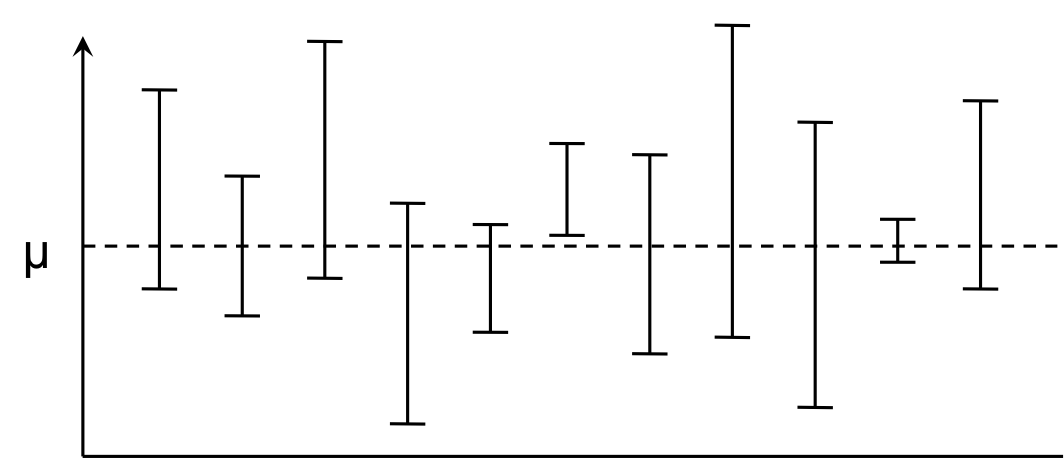
\includegraphics[width=0.7\textwidth]{figures/CI.png}
\end{figure}
\end{frame}


%-------------------
\begin{frame}{CI for the Mean: Known Variance}
$(\bar X - \frac{1.96 \sigma}{\sqrt{n}},\bar X + \frac{1.96 \sigma}{\sqrt{n}})$ is 
a CI for $\mu$ with confidence level $0.95$.
\begin{itemize}
\item Problem: need to know the population variance $\sigma^2$.
\item Unfortunately, the assumption that $\sigma^2$ is known is unrealistic in many situations. 
\item Solution: in practice, we typically use $S^2$, the sample variance, to estimate it.
\[
S^2 = \frac{1}{n-1} \sum_{i=1}^n (X_i - \bar X)^2
\]
\end{itemize}
\end{frame}

%-------------------
\begin{frame}{CI for the Mean: \alert{Unknown} Variance}
Consider the random variable
\[
T = \frac{\bar X - \mu} {S / \sqrt{n}}.
\]

Why it is a random variable?
\begin{itemize}
\item The observations $X_1,\cdots,X_n$ are random.
\item Thus, the sample mean $\bar X$ and sample variance $S^2$ are random;
\item Thus, the ratio $T$ is random.
\end{itemize}

\end{frame}

%-------------------
\begin{frame}{CI for the Mean: Unknown Variance}
\begin{block}{Distribution of $T$}
If $\bar X$ is normally distributed, then 
\[T = \frac{\bar X - \mu} {S / \sqrt{n}} \]
follows a \alert{Student's t-distribution} with $n-1$ degrees of freedom. 
\end{block}
\vspace{\stretch{0.3}}
When is $\bar X$ is normally distributed?
\begin{itemize}
\item The observations $X_1,\cdots,X_n$ are drawn independently from the population.
\item Either the population is normal, or sample size $n\geq 30$.
\end{itemize}
\end{frame}

%-------------------
\begin{frame}{The t-Distribution}
\begin{itemize}
\item The t-distribution is ``similar'' to the standard normal distribution.
\item It is continuous, bell-shaped, and symmetric around zero, but it has fatter tails than the standard normal distribution.
\item The t-distribution has one parameter, the degrees of freedom (df).
\end{itemize}
\end{frame}

%-------------------
\begin{frame}{The t-Distribution}
\begin{figure}
    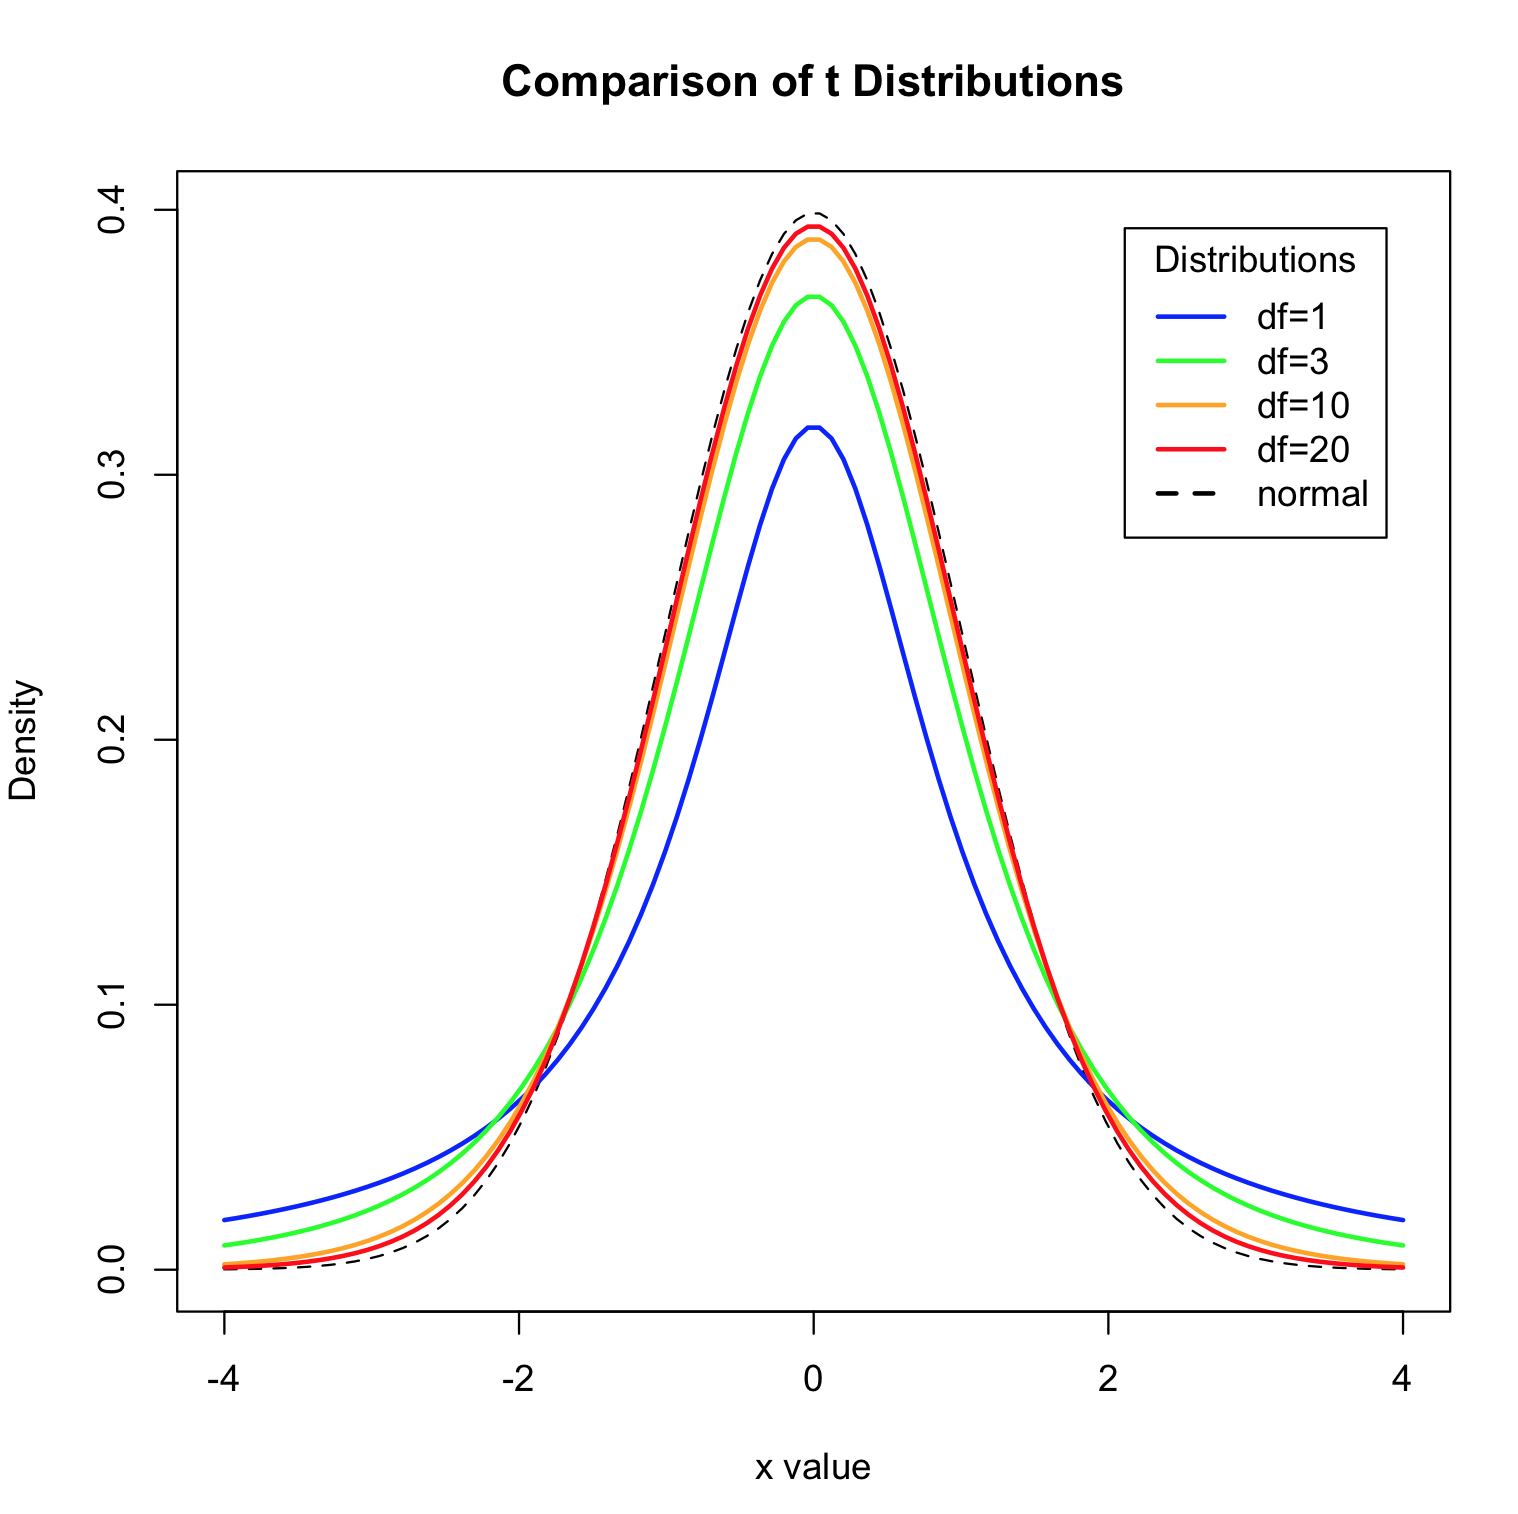
\includegraphics[width=0.7\textwidth]{figures/t_pdf.png}
\end{figure}
\end{frame}

%-------------------
\begin{frame}{The t- Distribution}
\begin{itemize}
\item When the df is large (df $\geq 30$), the t-distribution is close to the standard normal distribution $Z$.
\item As df $\to\infty$, the t-distribution converges to the standard normal distribution $Z$.
\end{itemize}
\end{frame}

%-------------------
\begin{frame}{The t-Distribution}
Notation $t_{\alpha,\nu}$: the point that the area to its right under the t-distribution curve with df=$\nu$ is $\alpha$, thus
$$\pr(-t_{\alpha,\nu} \leq T \leq t_{\alpha,\nu}) = 1-2\alpha.$$
\begin{center}
    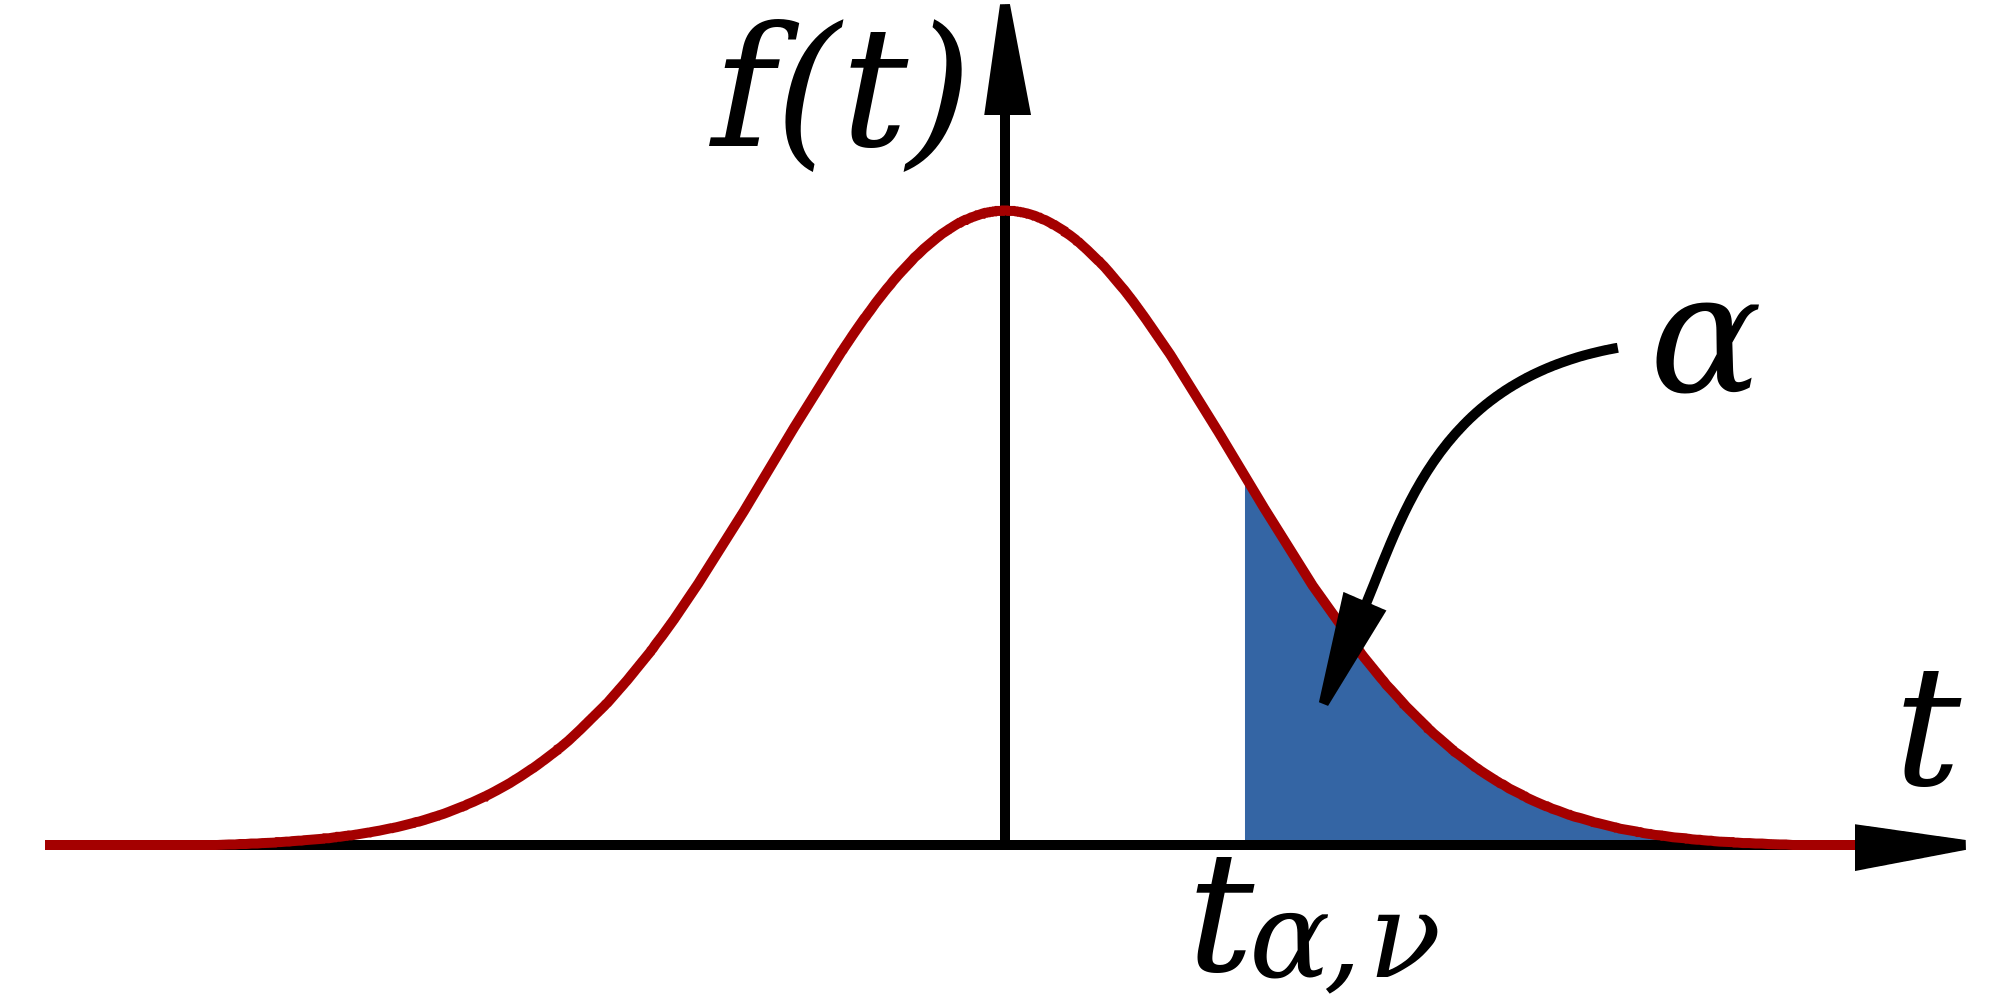
\includegraphics[width=0.5\textwidth]{figures/t_tail.png}
\end{center}

\begin{itemize}
\item Use t-table to find $t_{\alpha,\nu}$, for different $\alpha$,$\nu$.
\item Example: What is $t_{0.05, 19}$?  What is $t_{0.025, 9}$? 
\end{itemize}
\end{frame}


%-------------------
\begin{frame}{CI for the Mean: Unknown Variance}
A $1-\alpha$ CI for $\mu$ is ...
\begin{itemize}
\item When $n$ is large $(n\geq 30)$, approximate $T$ with $Z$:
\begin{align*}
 & \pr(-\textcolor{red}{z_{\alpha/2}} \leq \frac{\bar X - \mu}{S/\sqrt{n}} \leq \textcolor{red}{z_{\alpha/2}})=1-\alpha \\
& \Rightarrow \pr(\bar X -{z_{\alpha/2}} \frac{S}{\sqrt{n}} \leq \mu \leq \bar X +{z_{\alpha/2}} \frac{S}{\sqrt{n}})=1-\alpha.
\end{align*}
\item When $n$ is small and the population is normal:
\begin{align*}
 & \pr(-\textcolor{red}{t_{\alpha/2,n-1}} \leq \frac{\bar X - \mu}{S/\sqrt{n}} \leq \textcolor{red}{t_{\alpha/2,n-1}})=1-\alpha \\
& \Rightarrow \pr(\bar X -{t_{\alpha/2,n-1}} \frac{S}{\sqrt{n}} \leq \mu \leq \bar X +{t_{\alpha/2,n-1}} \frac{S}{\sqrt{n}})=1-\alpha.
\end{align*}
\end{itemize}
\end{frame}

%-------------------
\begin{frame}{CI for the Mean: Summary}
 \begin{table}
 \begin{center}
 \begin{tabular}{|M{3cm}|M{3cm}|M{3cm}|N}
 \hline
  & $\sigma \text{ known}$ & $\sigma \text{ unknown}$ \\[5pt]\hline
 $n\geq 30$ & 
$$ \bar X \pm z_{\alpha/2} \frac{\sigma}{\sqrt{n}}$$ & 
$$ \bar X \pm z_{\alpha/2} \frac{S}{\sqrt{n}}$$  \\[20pt] \hline
 $n< 30$, pop. is normal &  
$$ \bar X \pm z_{\alpha/2} \frac{\sigma}{\sqrt{n}} $$& 
$$ \bar X \pm \textcolor{red}{t_{\alpha/2,n-1}} \frac{S}{\sqrt{n}}$$  \\ [20pt]\hline
$n< 30$, pop. isn't normal & 
 N.A. & N.A. \\ \hline
 \end{tabular}
 \end{center}
 \end{table}
\end{frame}

%-------------------
\begin{frame}{Degrees of Freedom (df)}
The random variable $S$ computed with $n$ observations has degrees of freedom $n-1$.
\[
S^2 = \frac{1}{n-1} \sum_{i=1}^n (X_i - \bar X)^2.
\]

Proof sketch: define random variables $Y_i = X_i - \bar X$. Then,
$S^2 = \frac{1}{n-1} \sum_{i=1}^n Y_i^2$.
However, $Y_i$ must satisfy one restriction: 
\[\sum_{i=1}^n Y_i = (\sum_{i=1}^n X_i) - n \bar X = 0.
\]
Thus $S^2$ loses one degree of ``freedom''.\qed

\let\thefootnote\relax\footnotetext{\tiny{* Note: the definition of df is not required for this class.}}
\end{frame}


%-------------------
\begin{frame}{CI for the Proportion}
Often interested to know the proportion of the population that satisfies a condition, e.g.
\begin{itemize}
\item Proportion of NYU undergrads owning an iPhone;
\item Proportion of voters supporting candidate A.
\end{itemize}

\vspace{\stretch{0.2}}
Notation
\begin{itemize}
\item $p$ = proportion in population (population parameter)
\item $\h p$  = proportion in sample (sample statistic)
\end{itemize}

\vspace{\stretch{0.2}}
Goal: construct a confidence interval for $p$.
\end{frame}


%-------------------
\begin{frame}{CI for the Proportion}
Assume $X_1,\cdots,X_n$ are drawn indepedently from the population. Each $X_i$ is a random variable, with
\[
X_i=\begin{cases}
0, \quad \text{with prob. } 1- p\\
        1, \quad \text{with prob. }  p
        \end{cases}
\]
Then by definition,
\begin{align*}
\E (X_i) &= p \\
\var (X_i) & = (1-p) (0 -p)^2 + p (1-p)^2 = p(1-p)
\end{align*}
\end{frame}

%-------------------
\begin{frame}{CI for the Proportion}
The sample proportion is also a sample mean:
\[
\h p=\frac{1}{n} \sum_{i=1}^n X_i.
\]
By CLT,
\begin{itemize}
\item $\mu_{\h p} := \E (\h p) = p $.
\item $\sigma^2_{\h p} := \var (\h p)  = \frac{p(1-p)}{n}$.
\item When $n$ is large, $\h p$ is normally distributed.
\begin{itemize}
\item Here we need $np\geq 15$ and $n(1-p)\geq 15$.
\end{itemize}
\end{itemize}
\let\thefootnote\relax\footnotetext{\tiny{* ``$:=$'' means ``is defined as''.}}
\end{frame}

%-------------------
\begin{frame}{CI for the Proportion}
When $np\geq 15$ and $n(1-p)\geq 15$,
\begin{align*}
 & \pr(-z_{\alpha/2} \leq \frac{\h p - p }{\sigma_{\h p}}  \leq z_{\alpha/2}) = 1-\alpha\\
\Rightarrow \, & \pr(\h p - z_{\alpha/2}\, \sigma_{\h p} \leq p \leq 
 \h p + z_{\alpha/2} \,\sigma_{\h p} ) = 1-\alpha
\end{align*}

\begin{itemize}
\item $\sigma_{\h p} = \sqrt{\frac{p(1-p)}{n}}$, use $\sqrt{\frac{\h p(1-\h p)}{n}}$ as an approximation. 
\item Thus, a $1-\alpha$ confidence interval for population proportion $p$ is 
\[
\left( \h p - z_{\alpha/2} \sqrt{\frac{\h p(1-\h p)}{n}},\, 
 \h p + z_{\alpha/2} \sqrt{\frac{\h p(1-\h p)}{n}}\right)
\]
\end{itemize}
\end{frame}

%-------------------
\begin{frame}{Hypothesis Testing}
Often, someone makes a claim about the world, such as 
\begin{itemize}
\item A Mini Cooper achieve 37 highway miles per gallon.
\item AT\&T is the nation’s fastest 4G LTE network.
\item A Subway footlong sub is 12 inches long.
\end{itemize}

\vspace{\stretch{0.2}}
We collect some data, and we want to evaluate the plausibility of that claim in the face of data.
\end{frame}

%-------------------
\begin{frame}{Hypothesis Testing}
Common use cases for hypothesis testing:
\begin{itemize}
\item Check stated claims, e.g. model is realistic.
\item Check if possible that something happens by chance alone, e.g. 10 heads in a roll by a fair coin.
\item Check for effects of an intervention, e.g. A/B testing. 
\end{itemize}
\end{frame}

%-------------------
\begin{frame}{Hypothesis Testing}
%Hypothesis:
%\begin{itemize}
%\item  A statement about the numerical value of a population parameter.
%\end{itemize}
%\vspace{\stretch{0.2}}
Null Hypothesis ($H_0$):
\begin{itemize}
\item The hypothesis that will be accepted unless the data provide convincing evidence that it is false.
\item Example: stated claim is true; event occurs by chance; the intervention has no effect.
\end{itemize}
\vspace{\stretch{0.2}}
Alternative Hypothesis ($H_A$):
\begin{itemize}
\item The hypothesis that will be accepted when the null hypothesis is rejected. %data provide convincing evidence of its truth.
\item Example:  stated claim is false; event doesn't occurs by chance alone; the intervention has effect.
\end{itemize}
\end{frame}

%-------------------
\ignore{
\begin{frame}{Time Series Plot}
\begin{figure}
    \caption{}
    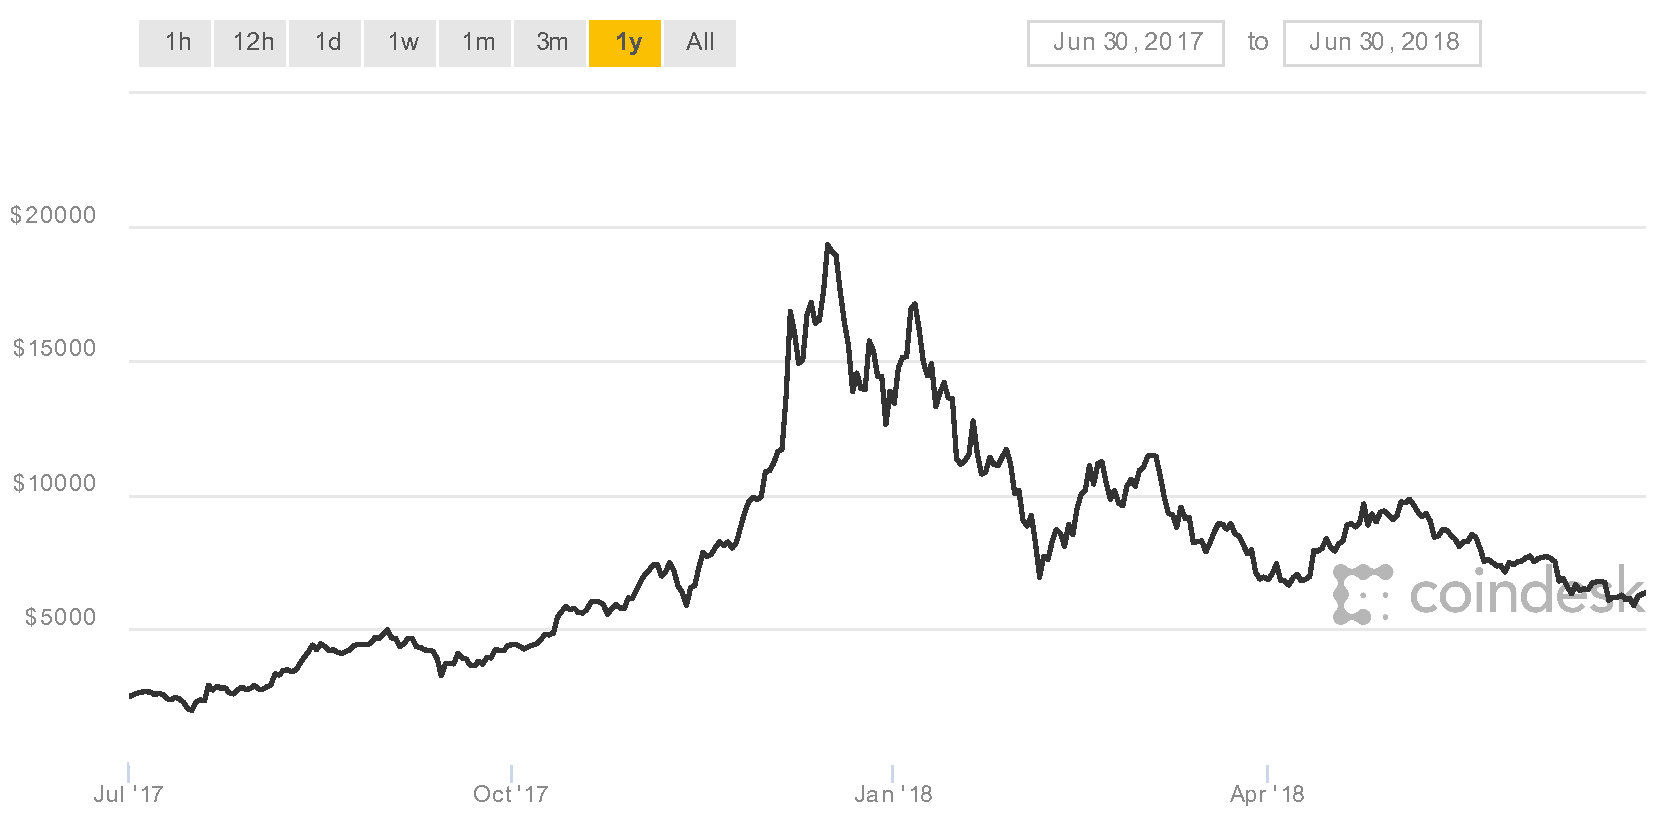
\includegraphics[width=1\textwidth]{figures/coindesk-bpi-chart}
\end{figure}
\let\thefootnote\relax\footnotetext{\tiny{* Plot from Coindesk.com}}
\end{frame}

\begin{frame}{}
\begin{itemize}
\item 
\end{itemize}
\end{frame}

\vspace{\stretch{0.5}}

\begin{block}{}
\end{block}


}

\end{document}


